\documentclass{beamer}
\usepackage{amsmath}
\usepackage[english]{babel} %set language; note: after changing this, you need to delete all auxiliary files to recompile
\usepackage[utf8]{inputenc} %define file encoding; latin1 is the other often used option
\usepackage{csquotes} % provides context sensitive quotation facilities
\usepackage{graphicx} %allows for inserting figures
\usepackage{booktabs} % for table formatting without vertical lines
\usepackage{textcomp} % allow for example using the Euro sign with \texteuro
\usepackage{stackengine}
\usepackage{wasysym}
\usepackage{tikzsymbols}
\usepackage{textcomp}
\newcommand{\bubblethis}[2]{
        \tikz[remember picture,baseline]{\node[anchor=base,inner sep=0,outer sep=0]%
        (#1) {\underline{#1}};\node[overlay,cloud callout,callout relative pointer={(0.2cm,-0.7cm)},%
        aspect=2.5,fill=yellow!90] at ($(#1.north)+(-0.5cm,1.6cm)$) {#2};}%
    }%
\tikzset{face/.style={shape=circle,minimum size=4ex,shading=radial,outer sep=0pt,
        inner color=white!50!yellow,outer color= yellow!70!orange}}
%% Some commands to make the code easier
\newcommand{\emoticon}[1][]{%
  \node[face,#1] (emoticon) {};
  %% The eyes are fixed.
  \draw[fill=white] (-1ex,0ex) ..controls (-0.5ex,0.2ex)and(0.5ex,0.2ex)..
        (1ex,0.0ex) ..controls ( 1.5ex,1.5ex)and( 0.2ex,1.7ex)..
        (0ex,0.4ex) ..controls (-0.2ex,1.7ex)and(-1.5ex,1.5ex)..
        (-1ex,0ex)--cycle;}
\newcommand{\pupils}{
  %% standard pupils
  \fill[shift={(0.5ex,0.5ex)},rotate=80] 
       (0,0) ellipse (0.3ex and 0.15ex);
  \fill[shift={(-0.5ex,0.5ex)},rotate=100] 
       (0,0) ellipse (0.3ex and 0.15ex);}

\newcommand{\emoticonname}[1]{
  \node[below=1ex of emoticon,font=\footnotesize,
        minimum width=4cm]{#1};}
\usepackage{scalerel}
\usetikzlibrary{positioning}
\usepackage{xcolor,amssymb}
\newcommand\dangersignb[1][2ex]{%
  \scaleto{\stackengine{0.3pt}{\scalebox{1.1}[.9]{%
  \color{red}$\blacktriangle$}}{\tiny\bfseries !}{O}{c}{F}{F}{L}}{#1}%
}
\newcommand\dangersignw[1][2ex]{%
  \scaleto{\stackengine{0.3pt}{\scalebox{1.1}[.9]{%
  \color{red}$\blacktriangle$}}{\color{white}\tiny\bfseries !}{O}{c}{F}{F}{L}}{#1}%
}
\usepackage{fontawesome} % Social Icons
\usepackage{epstopdf} % allow embedding eps-figures
\usepackage{tikz} % allows drawing figures
\usepackage{amsmath,amssymb,amsthm} %advanced math facilities
\usepackage{lmodern} %uses font that support italic and bold at the same time
\usepackage{hyperref}
\usepackage{tikz}
\usepackage{tcolorbox}
\usetikzlibrary{patterns}

\usefonttheme[onlymath]{serif} %set math font to serif ones

\definecolor{beamerblue}{rgb}{0.2,0.2,0.7} %define beamerblue color for later use

%%% defines highlight command to set text blue
\newcommand{\highlight}[1]{{\color{blue}{#1}}}


%%%%%%% commands defining backup slides so that frame numbering is correct

\newcommand{\backupbegin}{
   \newcounter{framenumberappendix}
   \setcounter{framenumberappendix}{\value{framenumber}}
}
\newcommand{\backupend}{
   \addtocounter{framenumberappendix}{-\value{framenumber}}
   \addtocounter{framenumber}{\value{framenumberappendix}}
}

%%%% end of defining backup slides

%Specify figure caption, see also http://tex.stackexchange.com/questions/155738/caption-package-not-working-with-beamer
\setbeamertemplate{caption}{\insertcaption} %redefines caption to remove label "Figure".
%\setbeamerfont{caption}{size=\scriptsize,shape=\itshape,series=\bfseries} %sets figure  caption bold and italic and makes it smaller


\usetheme{Boadilla}


% --------------------
% Overall information
% --------------------
\title[Economía I]{Economía I \vspace{4mm}
\\ Magistral 15: Distorsiones de mercado I}
\date{}
\author[Ertola Navajas y Fariña]{Ertola Navajas y Fariña}
\vspace{0.4cm}
\institute[]{Universidad de San Andrés} 

\begin{document}

\begin{frame}
\titlepage
\centering
\includegraphics[scale=0.2]{../Figures/logoUDESA.jpg} 
\end{frame}

\begin{frame}{Distorsiones al equilibrio de mercado}
    \begin{itemize}
        \item Creadas por el hombre:
        \begin{itemize}
            \item Impuestos
             \vspace{1mm}
            \item Precios máximos o mínimos (cepo)
             \vspace{1mm}
            \item Regulación (ley de alquileres)
            \vspace{1mm}
            \item Monopolios artificiales (farmacias, escribanos, low cost)
        \end{itemize}
    \end{itemize}
\end{frame}

\begin{frame}{Precios máximos......}
\begin{itemize}
    \item ¿Motivos?
    \item Casos
    \item Consecuencias ¿Ganadores y perdedores?. El caso del termómetro
    \begin{itemize}
        \item Deja de ser una señal
        \item No soluciona el problema de fondo
        \item ¿Quien queda afuera?
    \end{itemize}
\end{itemize}
\end{frame}


\begin{frame}{Precios máximos......}
\includegraphics[scale=0.15]{../Figures/Precioscuidados.jpg}
\end{frame}


\begin{frame}{Precios máximos......}
\centering
\includegraphics[scale=0.45]{../Figures/Acuerdoprecios.jpg}
\end{frame}


\begin{frame}{Precios máximos......}
\centering
\includegraphics[scale=0.9]{../Figures/Dolar.jpg}
\end{frame}


\begin{frame}{Precios Máximos}
\begin{figure} [H]
\caption{Precio Máximo}
    \centering
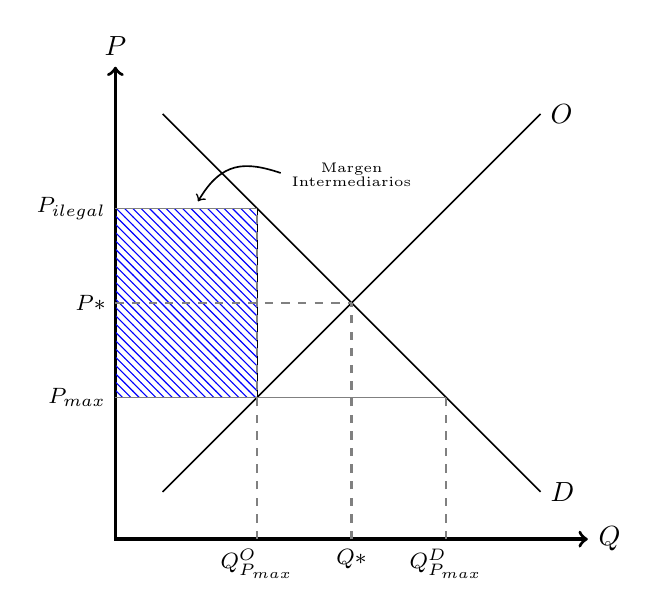
\begin{tikzpicture}[scale=0.6]
\draw[very thick,<->] (0,10) node[above]{$P$}--(0,0)--(10,0) node[right]{$Q$};
\draw[semithick](1,1)--(9,9) node[right]{$O$};
\draw [semithick] (1,9)--(9,1) node[right]{$D$};
\draw [pattern=north west lines, pattern color=blue] (0,3) rectangle (3,7);
\draw[thick, gray, dashed](3,0)--(3,7) ;
\draw[semithick, gray](0,3)--(7,3);
\draw[thick, gray, dashed](5,0)--(5,5) ;
\draw[thick, gray, dashed](0,5)--(5,5) ;
\draw[thick, gray, dashed](7,0)--(7,3) ;
\draw[semithick, gray](0,7)--(3,7);
%\draw[semithick, gray,dashed](3,3)--(7.5,3);
\node[left] at (0,3){\footnotesize $P_{max}$};
\node[left] at (0,7){\footnotesize $P_{ilegal}$};
\node[left] at (0,5){\footnotesize $P*$};
\node[below] at (5,0){\footnotesize $Q*$};
\node[below] at (3,0){\footnotesize $Q_{P_{max}}^{O}$};
\node[below] at (7,0){\footnotesize $Q_{P_{max}}^{D}$};
\draw[semithick, <-] (1.75,7.15).. controls (2.25,8) and (2.75,8).. (3.5,7.75);
\node[above] at (5,7.5) {\tiny Margen};
\node[above] at (5,7.25) {\tiny Intermediarios};
\end{tikzpicture}
\label{fig:20.6}
\end{figure}  
\end{frame}

\begin{frame}{Precios sostén}
\centering
\includegraphics[scale=0.5]{../Figures/Preciominimo.png}
\end{frame}


\begin{frame}{Precios sostén}
\begin{figure} [H]
\centering
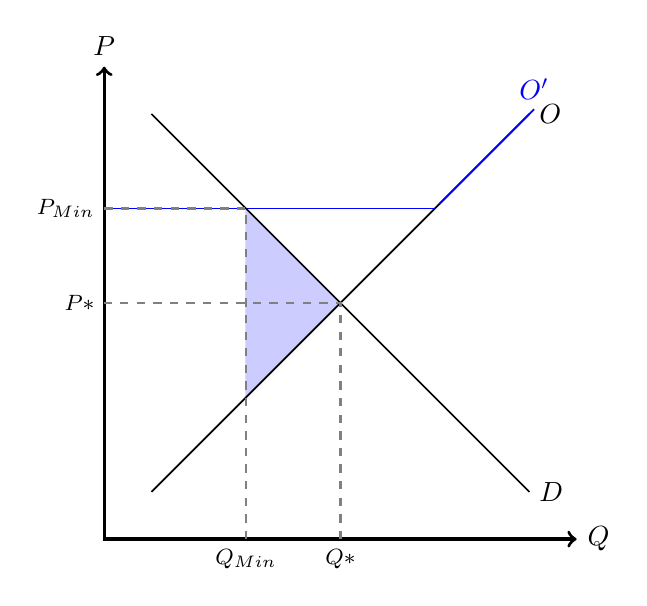
\begin{tikzpicture}[scale=0.6]
\draw[very thick,<->] (0,10) node[above]{$P$}--(0,0)--(10,0) node[right]{$Q$};
\draw[fill,blue!20] (5,5)--(3,7)--(3,3);
\draw [semithick](1,1)--(9,9) node[right]{$O$};
\draw [semithick, blue](7.1,7.1)--(9.1,9.1) node[above]{$O'$};
\draw [semithick, blue](7,7)--(0,7);
\draw [semithick](1,9)--(9,1) node[right]{$D$};
\draw[thick, gray, dashed](3,0)--(3,7) ;
\draw[thick, gray, dashed](0,7)--(3,7) ;
\draw[thick, gray, dashed](5,0)--(5,5)--(0,5) ;
%\node[left] at (0,3){\footnotesize $P^{'}_D$};
\node[left] at (0,7){\footnotesize $P_{Min}$};
\node[below] at (3,0){\footnotesize $Q_{Min}$};
\node[left] at (0,5){\footnotesize $P*$};
\node[below] at (5,0){\footnotesize $Q*$};
\end{tikzpicture}
\label{fig:20.7}
\end{figure} 
\end{frame}

\begin{frame}{Precios sostén con mercado paralelo}
\begin{figure} [H]
\centering
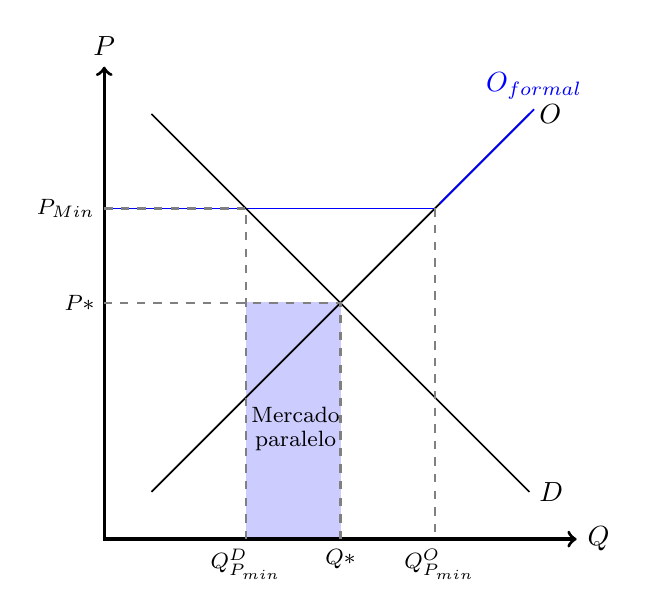
\begin{tikzpicture}[scale=0.6]
\draw[very thick,<->] (0,10) node[above]{$P$}--(0,0)--(10,0) node[right]{$Q$};
\draw[fill,blue!20] (3,0.05)--(5,0.05)--(5,5)--(3,5);
\draw [semithick](1,1)--(9,9) node[right]{$O$};
\draw [semithick, blue](7.1,7.1)--(9.1,9.1) node[above]{$O_{formal}$};
\draw [semithick, blue](7,7)--(0,7);
\draw [semithick](1,9)--(9,1) node[right]{$D$};
\draw[thick, gray, dashed](3,0)--(3,7) ;
\draw[thick, gray, dashed](0,7)--(3,7) ;
%\draw[thick, gray, dashed](0,7)--(7,7)--(7,3)--(0,3) ;
\draw[thick, gray, dashed](5,0)--(5,5)--(0,5) ;
\draw[thick, gray, dashed](7,7)--(7,0) ;
%\node[left] at (0,3){\footnotesize $P^{'}_D$};
\node[left] at (0,7){\footnotesize $P_{Min}$};
\node[below] at (3,0){\footnotesize $Q_{P_{min}}^{D}$};
\node[below] at (7.1,0){\footnotesize $Q_{P_{min}}^{O}$};
\node[left] at (0,5){\footnotesize $P*$};
\node[below] at (5,0){\footnotesize $Q*$};
\node[below] at (4.05,3){\footnotesize Mercado};
\node[below] at (4.05,2.5){\footnotesize paralelo};
\end{tikzpicture}
\label{fig:20.7b}
\end{figure}  
\end{frame}

\begin{frame}{Precios sostén con adquisición del excedente}
\begin{figure} [H]
\caption{Sin reventa}
\centering
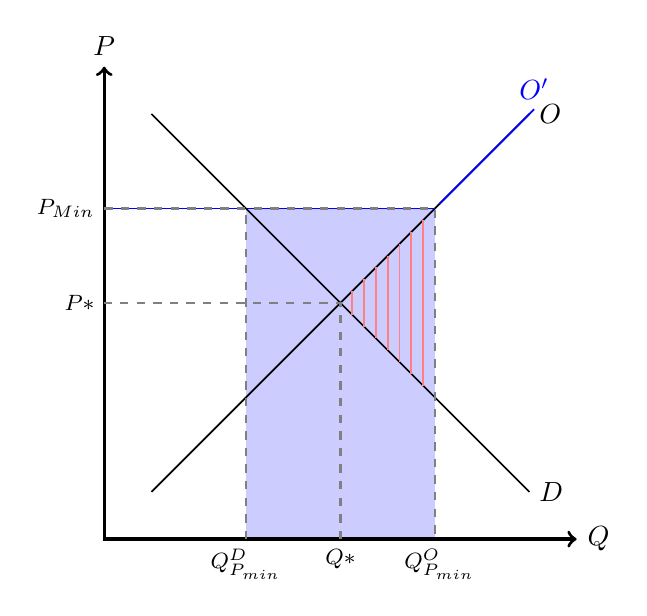
\begin{tikzpicture}[scale=0.6]
\draw[very thick,<->] (0,10) node[above]{$P$}--(0,0)--(10,0) node[right]{$Q$};
\draw[fill,blue!20] (3,0.05)--(7,0.05)--(7,7)--(3,7);
\draw [semithick](1,1)--(9,9) node[right]{$O$};
\draw [semithick, blue](7.1,7.1)--(9.1,9.1) node[above]{$O'$};
\draw [semithick, blue](7,7)--(0,7);
\draw [semithick](1,9)--(9,1) node[right]{$D$};
\draw[semithick, red!50] (6.75,3.25)--(6.75,6.75);
\draw[semithick, red!50] (6.5,3.5)--(6.5,6.5);
\draw[semithick, red!50] (6.25,3.75)--(6.25,6.25);
\draw[semithick, red!50] (6,4)--(6,6);
\draw[semithick, red!50] (5.75,4.25)--(5.75,5.75);
\draw[semithick, red!50] (5.5,4.5)--(5.5,5.5);
\draw[semithick, red!50] (5.25,4.75)--(5.25,5.25);
%\draw[thick, gray, dashed](2,0)--(2,7) ;
\draw[thick, gray, dashed](0,7)--(2,7) ;
\draw[thick, gray, dashed](0,7)--(7,7)--(7,0) ;
\draw[thick, gray, dashed](5,0)--(5,5)--(0,5) ;
\draw[thick, gray, dashed](3,0)--(3,7);
\node[left] at (0,7){\footnotesize $P_{Min}$};
\node[below] at (3,0){\footnotesize $Q_{P_{min}}^{D}$};
\node[below] at (7.1,0){\footnotesize $Q_{P_{min}}^{O}$};
\node[left] at (0,5){\footnotesize $P*$};
\node[below] at (5,0){\footnotesize $Q*$};
\end{tikzpicture}
\label{fig:20.7c}
\end{figure} 

\end{frame}

\begin{frame}{Precios sostén con adquisición del excedente}
\begin{figure} [H]
\caption{Con reventa}
\centering
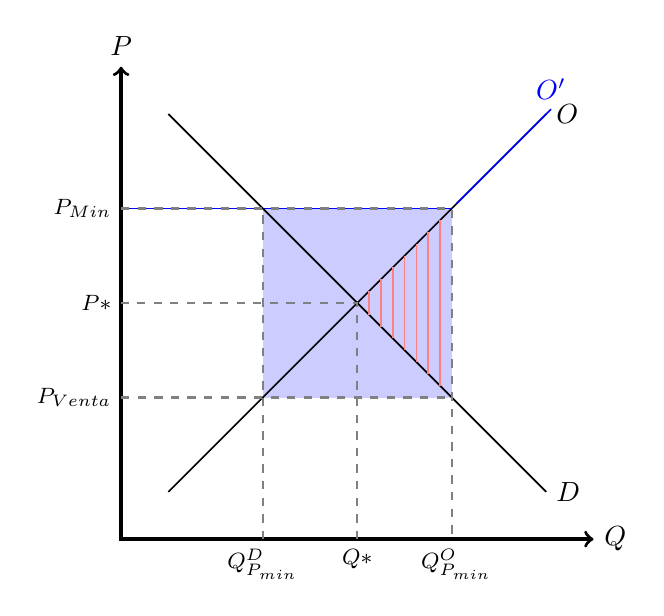
\begin{tikzpicture}[scale=0.6]
\draw[very thick,<->] (0,10) node[above]{$P$}--(0,0)--(10,0) node[right]{$Q$};
\draw[fill,blue!20] (3,3)--(7,3)--(7,7)--(3,7);
\draw [semithick](1,1)--(9,9) node[right]{$O$};
\draw [semithick, blue](7.1,7.1)--(9.1,9.1) node[above]{$O'$};
\draw [semithick, blue](7,7)--(0,7);
\draw [semithick](1,9)--(9,1) node[right]{$D$};
\draw[semithick, red!50] (6.75,3.25)--(6.75,6.75);
\draw[semithick, red!50] (6.5,3.5)--(6.5,6.5);
\draw[semithick, red!50] (6.25,3.75)--(6.25,6.25);
\draw[semithick, red!50] (6,4)--(6,6);
\draw[semithick, red!50] (5.75,4.25)--(5.75,5.75);
\draw[semithick, red!50] (5.5,4.5)--(5.5,5.5);
\draw[semithick, red!50] (5.25,4.75)--(5.25,5.25);
%\draw[thick, gray, dashed](2,0)--(2,7) ;
\draw[thick, gray, dashed](0,7)--(2,7) ;
\draw[thick, gray, dashed](0,7)--(7,7)--(7,0) ;
\draw[thick, gray, dashed](5,0)--(5,5)--(0,5) ;
\draw[thick, gray, dashed](3,0)--(3,7) ;
\draw[thick, gray, dashed](0,3)--(7,3) ;
%\node[left] at (0,3){\footnotesize $P^{'}_D$};
\node[left] at (0,7){\footnotesize $P_{Min}$};
\node[left] at (0,3){\footnotesize $P_{Venta}$};
\node[below] at (3,0){\footnotesize $Q_{P_{min}}^{D}$};
\node[below] at (7.1,0){\footnotesize $Q_{P_{min}}^{O}$};
\node[left] at (0,5){\footnotesize $P*$};
\node[below] at (5,0){\footnotesize $Q*$};
\end{tikzpicture}
\label{fig:20.7c}
\end{figure} 
\end{frame}

%\begin{frame}{15. El mercado de Berlín}
%    \begin{figure}[htp]
%\href{https://twitter.com/andreaskluth/status/1366691926804754440} {\makebox[\textwidth][c]{\includegraphics[width=0.45\textwidth]{images/TW.1.png}}} 
%\end{figure}
%Son muchos tweet en un imagen y para que entre todo queda muy chico. Igual haciendo click te lleva al hilo.
%\end{frame}

\begin{frame}{Distorsiones del Monopolio}
\begin{figure} [H]
\centering
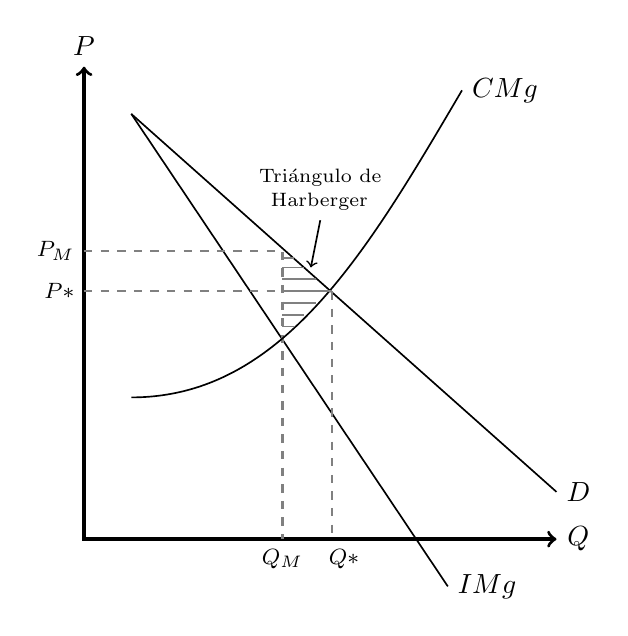
\begin{tikzpicture}[scale=0.6]
\draw[very thick,<->] (0,10) node[above]{$P$}--(0,0)--(10,0) node[right]{$Q$};
\draw[semithick](1,9)--(10,1) node[right]{$D$};
\draw[semithick](1,9)--(7.7,-1) node[right]{$IMg$};
\draw[thick,dashed,gray](0,6.1)--(4.2,6.1)--(4.2,0);
\draw[thick,dashed,gray](0,5.25)--(5.25,5.25)--(5.25,0);
%\draw(1,1)--(9,9);
\draw[semithick](1,3).. controls (4.2,3) and (6,6.1)..(8,9.5) node[right]{$CMg$};
\draw[semithick, gray] (4.2,5.95) to (4.45,5.95) ;
\draw[semithick, gray] (4.2,5.75) to (4.65,5.75) ;
\draw[semithick, gray] (4.2,5.5) to (4.9,5.5) ;
\draw[semithick, gray] (4.2,5.25) to (5.25,5.25) ;
\draw[semithick, gray] (4.2,5) to (4.9,5) ;
\draw[semithick, gray] (4.2,4.75) to (4.65,4.75) ;
\draw[semithick, gray] (4.2,4.5) to (4.45,4.5) ;
 \node [right] at (3.5,7.65) {\scriptsize Triángulo de};
 \node [right] at (3.75,7.15) {\scriptsize Harberger};
\draw[semithick, <-] (4.8,5.75)--(5,6.75);
\node[below] at(4.2,0) {\footnotesize $Q_M$};
\node[below] at(5.5,0) {\footnotesize $Q*$};
\node[left] at(0,6.1) {\footnotesize $P_{M}$};
\node[left] at(0,5.25) {\footnotesize $P*$};
\end{tikzpicture}
\label{fig:20.4}
\end{figure}
\end{frame}

  \begin{frame}{¿Eliminar al monopolio?}
    \begin{itemize}
        \item Lo primero que hay que hacer es entender porque hay un monopolio
        \item Y tratar de eliminarlo
        \item ¿Alcanza con decir que una empresa es grande para definir un monopolio? 
        \item No! ... si los mercados son contestables
        \item Solo en casos extremos debiéramos apelar a la regulación de precios
    \end{itemize}
\end{frame}

\begin{frame}{¿Cómo podemos regular un monopolio?}
\begin{figure} [H]
\caption{Precio Máximo en P*}
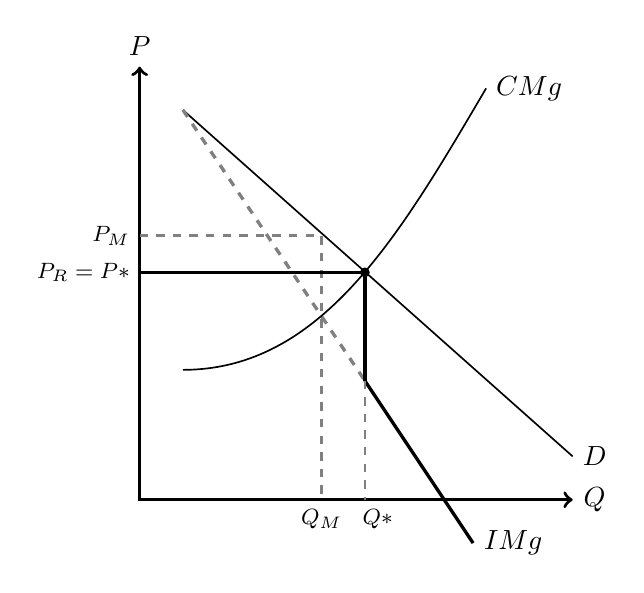
\begin{tikzpicture}[scale=0.55]
\draw[very thick,<->] (0,10) node[above]{$P$}--(0,0)--(10,0) node[right]{$Q$};
\draw[semithick](1,9)--(10,1) node[right]{$D$};
%\draw[semithick](1,9)--(7.7,-1) node[right]{$IMg$};
\draw[very thick,dashed,gray](1,9)--(5.2,2.75);
\draw[very thick](5.2,2.75)--(7.7,-1) node[right]{$IMg$};
\draw[thick,dashed,gray](5.2,2.75)--(5.2,0);
\draw[thick,dashed,gray](0,6.1)--(4.2,6.1)--(4.2,0);
\draw[very thick](0,5.25)--(5.2,5.25)--(5.2,2.75);
%\draw(1,1)--(9,9);
\draw[semithick](1,3).. controls (4.2,3) and (6,6.1)..(8,9.5) node[right]{$CMg$};
\node[below] at(4.2,0) {\footnotesize $Q_M$};
\node[below] at(5.5,0) {\footnotesize $Q*$};
\node[left] at(0,6.1) {\footnotesize $P_{M}$};
\node[left] at(0,5.25) {\footnotesize $P_{R}=P*$};
\draw[fill](5.2,5.25) circle [radius =0.1];
    \end{tikzpicture}
\label{fig:20.5}
\end{figure} 

\end{frame}


\begin{frame}{Monopolio Natural}
\begin{figure} [H]
\centering
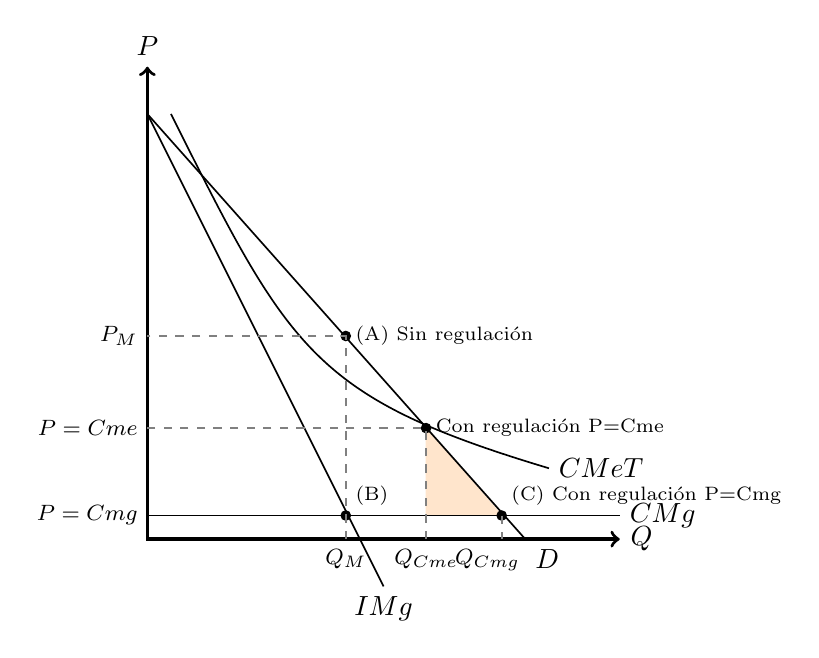
\begin{tikzpicture}[scale=0.6]
\draw[very thick,<->] (0,10) node[above]{$P$}--(0,0)--(10,0) node[right]{$Q$};
\draw[fill,orange!20]
(5.9,0.5)--(5.9,2.35)--(7.5,0.5);


\node[left] at (0,4.3) {\footnotesize $P_M$};
\node[below] at (4.2,0) {\footnotesize $Q_M$};
\node[left] at (0,2.35) {\footnotesize $P={Cme}$};
\node[below] at (5.9,0) {\footnotesize $Q_{Cme}$};
\node[left] at (0,0.5) {\footnotesize $P={Cmg}$};
\node[below] at (7.2,0) {\footnotesize $Q_{Cmg}$};


\draw[fill] (4.2,4.3) circle [radius =0.1] node[right] {\scriptsize (A) Sin regulación};
\draw[fill] (5.9,2.35) circle [radius =0.1] node[right] {\scriptsize Con regulación P=Cme};
\draw[fill] (7.5,0.5) circle [radius =0.1] node[above right] {\scriptsize (C) Con regulación P=Cmg};
\draw[fill] (4.2,0.5) circle [radius =0.1] node[above right] {\scriptsize (B)};


\draw[semithick](0,9)--(8,0) node[below right]{$D$};
\draw[semithick](0,9)--(5,-1) node[below]{$IMg$};
\draw[semithick](0,0.5)--(10,0.5) node[right]{$CMg$};
\draw[semithick](0.5,9) ..controls (3,4) and (3.5,3) .. (8.5,1.5) node[right]{$CMeT$};

\draw[thick, dashed,gray] (4.2,0)--(4.2,4.3)--(0,4.3);
\draw[thick, dashed,gray] (5.9,0)--(5.9,2.35)--(0,2.35);
\draw[thick, dashed,gray] (7.5,0.5)--(7.5,0);

\end{tikzpicture}
\label{fig:MNN}
\end{figure} 
\end{frame}


\begin{frame}{Poniéndole precio a una carretera  I}
     \begin{figure} [h!]
    \centering
    \includegraphics[width=0.80\textwidth]{../Figures/Paseobajo.jpg}
    \caption{Paseo del bajo}
    \label{fig:}
\end{figure}
\end{frame}

\begin{frame}{Poniéndole precio a una carretera  II}
    \begin{figure} [H]
\centering
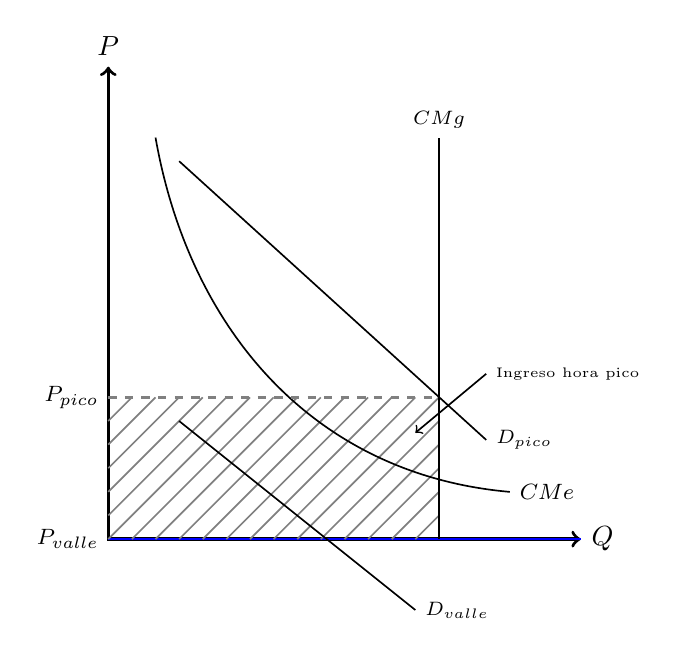
\begin{tikzpicture}[scale=0.6]
\draw[very thick,<->] (0,10) node[above]{$P$}--(0,0)--(10,0) node[right]{$Q$};
\draw[semithick, blue] (0,0)--(10,0);
\draw[semithick, gray] (0,2.5)--(0.5,3);
\draw[semithick, gray] (0,2)--(1,3);
\draw[semithick, gray] (0,1.5)--(1.5,3);
\draw[semithick, gray] (0,1)--(2,3);
\draw[semithick, gray] (0,0.5)--(2.5,3);
\draw[semithick, gray] (0,0)--(3,3);
\draw[semithick, gray] (0.5,0)--(3.5,3);
\draw[semithick, gray] (1,0)--(4,3);
\draw[semithick, gray] (1.5,0)--(4.5,3);
\draw[semithick, gray] (2,0)--(5,3);
\draw[semithick, gray] (2.5,0)--(5.5,3);
\draw[semithick, gray] (3,0)--(6,3);
\draw[semithick, gray] (3.5,0)--(6.5,3);
\draw[semithick, gray] (4,0)--(7,3);
\draw[semithick, gray] (4.5,0)--(7,2.5);
\draw[semithick, gray] (5,0)--(7,2);
\draw[semithick, gray] (5.5,0)--(7,1.5);
\draw[semithick, gray] (6,0)--(7,1);
\draw[semithick, gray] (6.5,0)--(7,0.5);
\draw [semithick] (1,8.5) to [out=280,in=175] (8.5,1)node [right] {\footnotesize $CMe$};
\draw [semithick] (7,0) to (7,8.5);
\node[above] at (7,8.5) {\scriptsize $CMg$};
\draw [semithick] (8,2.1) node [right]  {\scriptsize$D_{pico}$} to (1.5,8);
\draw [semithick] (6.5,-1.5) node [right]  {\scriptsize$D_{valle}$} to (1.5,2.5);
\draw[thick, gray, dashed](0,3)--(7,3) ;
\node[left] at (0,3){\footnotesize $P_{pico}$};
\node[left] at (0,0){\footnotesize $P_{valle}$};
\draw[semithick, ->] (8,3.5)--(6.5,2.25);
\node[right] at (8,3.5) {\tiny Ingreso hora pico};
\end{tikzpicture}
\label{fig:20.7}
\end{figure} 
 
\end{frame}

\begin{frame}{Regulaciones: Ley de alquileres. Dos mercados}

\end{frame}

\begin{frame}{Regulaciones: Escribanos / Farmacias (Q regulado)}

\end{frame}

\begin{frame}{Regulaciones: Traductores con precios regulados}

\end{frame}

\end{document}
